%% ============================================================
%%  CS 790 / 657 — Domain-Specific Programming for AI
%%  Final Project Report
%%  AttnFuse: An Embedded DSL for Compiling Attention Variants
%%             to Fused Triton GPU Kernels
%% ============================================================
\documentclass[10pt,twocolumn]{article}

\usepackage[margin=0.75in,top=0.9in,bottom=0.9in]{geometry}
\usepackage[T1]{fontenc}
\usepackage{lmodern}
\usepackage{microtype}
\usepackage{amsmath,amssymb}
\usepackage{graphicx}
\usepackage{booktabs}
\usepackage{multirow}
\usepackage{array}
\usepackage{float}
\usepackage{subcaption}
\usepackage{listings}
\usepackage{xcolor}
\usepackage[colorlinks=true,linkcolor=blue!60!black,
            citecolor=blue!60!black,urlcolor=blue!60!black]{hyperref}
\usepackage{parskip}
\usepackage{enumitem}
\usepackage{balance}

\definecolor{codebg}{HTML}{F8F8F8}
\definecolor{codeframe}{HTML}{CCCCCC}
\definecolor{kwcol}{HTML}{0000CC}
\definecolor{comcol}{HTML}{008000}
\definecolor{strcol}{HTML}{CC0000}
\lstset{
  language=Python,
  backgroundcolor=\color{codebg},
  frame=single,
  rulecolor=\color{codeframe},
  basicstyle=\ttfamily\scriptsize,
  keywordstyle=\color{kwcol}\bfseries,
  commentstyle=\color{comcol}\itshape,
  stringstyle=\color{strcol},
  numbers=left,
  numberstyle=\tiny\color{gray},
  numbersep=5pt,
  breaklines=true,
  showstringspaces=false,
  tabsize=4,
  captionpos=b,
}

\title{%
  \textbf{AttnFuse: An Embedded Python DSL for Compiling\\
  Attention Variants to Fused Triton GPU Kernels}\\[6pt]
  \normalsize CS 790/657: Domain-Specific Programming for AI --- Final Report
}
\author{Varun Kumar Dasoju}
\date{May 18, 2026}

\begin{document}
\maketitle

%% =============================================================
\begin{abstract}
%% =============================================================
Writing efficient GPU kernels for novel attention mechanisms is costly: each
new mask pattern, positional encoding, or bias scheme requires authoring and
tuning a new CUDA or Triton kernel from scratch.
\textbf{AttnFuse} is an embedded Python domain-specific language (DSL) that
solves this by letting the user \emph{declare} an attention variant using
composable combinators, then automatically compiling it to a single fused
Triton kernel via a two-level intermediate representation (IR) and a
compiler pipeline.
The compiler fuses the score, mask, bias, normalisation, and value-weighted
aggregation steps into one tiled loop that never materialises the full
$n \times n$ attention matrix in HBM, achieving IO-complexity identical to
hand-written FlashAttention-2.
On an NVIDIA RTX~3090 with fp16 inputs, AttnFuse matches PyTorch SDPA
within 8\% for dense and causal attention.
For variants not natively supported by SDPA---sliding-window (W=256) and
causal+ALiBi---AttnFuse achieves $61\times$ and $19\times$ speedup at
$N{=}4096$ over SDPA's $\mathcal{O}(n^2)$ fallback.
A novel fused Rotary Position Embedding (RoPE) kernel reduces end-to-end
latency by up to $2.3\times$ versus the pre-processing baseline.
All five attention variants are verified correct by 25 GPU unit tests.
\end{abstract}

%% =============================================================
\section{Introduction}
%% =============================================================

Modern Transformer architectures spend the majority of their compute and
memory budget inside multi-head self-attention.  Eager-mode PyTorch attention
launches multiple kernels---\texttt{Q@K\textsuperscript{T}}, scale, mask,
softmax, \texttt{attn@V}---and materialises the full $n \times n$ score
matrix in high-bandwidth memory (HBM), incurring $\mathcal{O}(n^2)$ memory
traffic quadratic in sequence length.  FlashAttention~\cite{dao2022flashattention,dao2023flashattention2}
eliminates this by fusing the entire attention loop and keeping
intermediate tiles in on-chip SRAM, reducing HBM reads from
$\mathcal{O}(n^2)$ to $\mathcal{O}(n^2 d / M)$ where $M$ is the SRAM size.

However, FlashAttention only handles a fixed set of variants (dense and
causal).  Research on long-range efficiency---sliding-window attention
\cite{child2019generating}, positional biases \cite{press2021alibi},
rotary embeddings \cite{su2021roformer}---requires writing new kernels
from scratch.  This is expensive: a production-quality Triton kernel with
proper tiling, pipeline staging, and mask logic takes weeks to write and tune.

\textbf{AttnFuse} provides a higher-level abstraction: the user writes a
short Python function using combinators (\texttt{causal}, \texttt{alibi},
\texttt{rope}, \texttt{softmax}, etc.), and the AttnFuse compiler
automatically generates a fused Triton kernel for any composition.

\paragraph{Contributions.}
\begin{itemize}[leftmargin=1.2em,itemsep=1pt]
  \item A composable DSL frontend with seven combinators, captured via
        symbolic tracing into a typed dataflow IR.
  \item A two-level IR design separating high-level combinator graphs from
        tiled-loop kernel records.
  \item A compiler pipeline (four passes) emitting a single parameterised
        Triton kernel specialised via \texttt{tl.constexpr} flags.
  \item A novel fused RoPE kernel that rotates Q/K tiles inside the inner
        loop, eliminating host-side preprocessing overhead.
  \item A complete evaluation covering five variants, three dtypes, four
        sequence lengths, and three baselines on RTX~3090.
\end{itemize}

%% =============================================================
\section{Background}
%% =============================================================

\subsection{FlashAttention and Online Softmax}

The key insight of FlashAttention is the \emph{online softmax}
algorithm~\cite{milakov2018online}: the numerically stable softmax can be
computed by maintaining running max $m_i$ and sum $\ell_i$ accumulators,
updating them as each key-value tile is loaded:
\begin{align*}
  m_\text{new} &= \max(m_i,\, \text{rowmax}(\mathbf{S})) \\
  \alpha        &= \exp(m_i - m_\text{new}) \\
  \mathbf{p}   &= \exp(\mathbf{S} - m_\text{new}) \\
  \ell_\text{new} &= \alpha\,\ell_i + \text{rowsum}(\mathbf{p}) \\
  \mathbf{acc}   &= \alpha\,\mathbf{acc} + \mathbf{p}\,\mathbf{V}
\end{align*}
This pattern allows the full attention computation---score, mask, bias,
normalise, aggregate---to be executed in a single nested loop over
$(M, N)$ tile coordinates, with only $\mathcal{O}(\text{SRAM})$ memory.

\subsection{Triton and JIT Specialisation}

Triton~\cite{tillet2019triton} is a Python-embedded DSL for GPU kernels that
compiles to PTX via LLVM.  Its \texttt{@triton.jit} decorator accepts
\texttt{tl.constexpr} arguments that are specialised at the Python level
before PTX code generation, enabling zero-overhead variant dispatch without
branching in the hot path.

\subsection{Rotary Position Embeddings}

RoPE~\cite{su2021roformer} encodes token position by rotating query and key
vectors by a position-dependent angle:
\[
  \mathbf{q}'_t = \mathbf{q}_t \odot \cos(\theta_t) +
                  \text{rotate\_half}(\mathbf{q}_t) \odot \sin(\theta_t)
\]
where $\text{rotate\_half}(\mathbf{x}) = [-x_{d/2:},\, x_{:d/2}]$.
Applying this before the attention dot product is equivalent to multiplying
scores by a relative-position phase factor, giving the model strong
relative position sensitivity without absolute position lookup tables.

%% =============================================================
\section{System Design}
%% =============================================================

\subsection{DSL Frontend}

AttnFuse exposes seven composable \emph{combinators}:

\begin{lstlisting}[caption={AttnFuse user code: GPT-2 style causal + ALiBi in 6 lines.}]
@af.attention
def gpt2_causal_alibi(Q, K, V):
    s = af.scaled_dot_product(Q, K)   # score
    s = af.alibi(s, num_heads=12)      # ALiBi bias
    s = af.causal(s)                   # causal mask
    p = af.softmax(s)                  # normalise
    return p @ V                       # aggregate
\end{lstlisting}

The \texttt{@af.attention} decorator traces the Python function once with
symbolic tensor arguments using a custom \texttt{TensorSym} class.
Each combinator call returns an IR node rather than a tensor, building a
dataflow graph that is captured without running any GPU code.

\subsection{Two-Level IR}

\paragraph{High-level IR.}
A \texttt{Graph} is a DAG of typed IR nodes:
\texttt{TensorSym} (leaves), \texttt{ScoreOp}, \texttt{MaskOp},
\texttt{BiasOp}, \texttt{NormOp}, and \texttt{MatMulPV} (root).
The graph is \emph{pure and symbolics}---no tensor data, only types and
structural information.  A SHA-1 hash of the graph's structural signature
serves as the process-local kernel cache key.

\paragraph{Tiled IR.}
The compiler lowers the DAG into a flat \texttt{TiledKernel} record
containing: \texttt{head\_dim}, \texttt{dtype}, \texttt{score\_scale},
\texttt{mask\_kind} (0/1/2), \texttt{bias\_kind} (0/1/2),
\texttt{norm\_kind} (0/1), \texttt{rope\_kind} (0/1),
and a \texttt{TileConfig} (BLOCK\_M, BLOCK\_N, num\_warps, num\_stages).
This separation cleanly decouples the user-facing graph semantics from
the tile-loop implementation details.

\subsection{Compiler Pipeline}

Four passes transform the high-level graph to a launched kernel:

\begin{enumerate}[leftmargin=1.5em,itemsep=1pt]
  \item \textbf{Fusion pass:} merges adjacent \texttt{ScoreOp} and
        \texttt{NormOp} nodes into the fused tile loop structure.
  \item \textbf{Tiling pass:} selects \texttt{BLOCK\_M},
        \texttt{BLOCK\_N}, \texttt{num\_warps}, and \texttt{num\_stages}
        from a hardware-tuned lookup table (Ampere sm\_86).
  \item \textbf{Lowering pass:} collapses the graph to a flat
        \texttt{TiledKernel} record.
  \item \textbf{Codegen pass:} returns a single kernel source string.
        Triton's \texttt{tl.constexpr} specialisation creates a distinct
        PTX binary for each unique (MASK\_KIND, BIAS\_KIND, NORM\_KIND,
        ROPE\_KIND, BLOCK\_M, BLOCK\_N, HEAD\_DIM) combination.
\end{enumerate}

Generated kernel sources are written to \texttt{attnfuse/\_generated/}
and cached both on disk (across process restarts) and in a process-local
\texttt{LaunchBundle} dictionary keyed by graph signature.

\subsection{Kernel Architecture}

The single generated kernel implements the tiled online-softmax loop with
all variants gated behind \texttt{tl.constexpr} branches.  For causal and
sliding-window masks, the inner loop bounds are trimmed to skip empty
$N$-blocks, reducing iteration count by up to $50\%$ for causal and
proportionally more for narrow sliding windows.

\paragraph{Fused RoPE.}
When \texttt{ROPE\_KIND\,==\,1}, the kernel:
(a) loads the Q tile, then loads a second Q tile at permuted head-dim
    offsets to compute $\text{rotate\_half}(\mathbf{Q})$ via a gather;
(b) applies $\mathbf{Q}' = \mathbf{Q} \odot \cos + \text{rh}(\mathbf{Q}) \odot \sin$
    in fp32 before the inner loop;
(c) loads the K tile and its rotated counterpart inside each inner-loop
    iteration and applies the same rotation.
This eliminates the two host-side \texttt{apply\_rope()} calls and avoids
one extra round-trip to HBM for the rotated query.

\paragraph{Sliding-window guard.}
All-masked inner blocks (where every query row has no keys within the
window) produce $\exp(-\infty - (-\infty)) = \text{NaN}$ in the online
softmax.  We gate the problematic division with an \texttt{all\_masked}
predicate derived from the block-level max, restoring correct accumulation.

%% =============================================================
\section{Implementation Details}
%% =============================================================

\subsection{Tile Size Selection}

The Ampere tile table (Table~\ref{tab:tile}) was derived by sweeping
$\text{BLOCK\_M} \in \{64,128\}$, $\text{BLOCK\_N} \in \{32,64\}$,
$\text{num\_warps} \in \{4,8\}$, $\text{num\_stages} \in \{2,3,4\}$
at $N{=}2048$ on the RTX~3090 (Section~\ref{sec:ablation}).
The RoPE variants use conservative $\text{num\_stages}=2$ to fit within
the 101\,KB usable SMEM after adding cos/sin tile loads.

\begin{table}[H]
\centering
\caption{Default Ampere tile configuration table (fp16/bf16).}
\label{tab:tile}
\small
\begin{tabular}{ccccc}
\toprule
\textbf{head\_dim} & \textbf{BM} & \textbf{BN} & \textbf{warps} & \textbf{stages} \\
\midrule
32  & 128 & 64 & 4 & 3 \\
64  & 128 & 64 & 4 & 3 \\
96  & 128 & 64 & 4 & 3 \\
128 & 128 & 32 & 8 & 2 \\
256 & 64  & 32 & 4 & 2 \\
\bottomrule
\end{tabular}
\end{table}

\subsection{Dispatch Overhead Optimisation}

A naive implementation recomputes constexpr dictionaries and allocates
placeholder tensors on every kernel call, adding $\sim$7\,$\mu$s of Python
overhead.  We precompute all dispatch metadata at compile time into a
\texttt{LaunchBundle} dataclass and cache placeholder slope/bias/rope tensors
using \texttt{functools.lru\_cache}, reducing per-call overhead to $<$1\,$\mu$s.

\subsection{Triton Compilation Pitfalls}

Two Triton 3.1 limitations required workarounds:
\begin{itemize}[leftmargin=1.2em,itemsep=1pt]
  \item \textbf{Compound constexpr:} \texttt{if A and B} where both are
        \texttt{tl.constexpr} fails silently (the body is never executed).
        Fixed by separating into \texttt{if A: ... elif B: ...} chains.
  \item \textbf{Source inspection:} the JIT requires reading the kernel
        source as a file (for LLVM to hash).  We write generated sources to
        \texttt{\_generated/} and import via \texttt{importlib.util}.
\end{itemize}

%% =============================================================
\section{Evaluation}
%% =============================================================

All experiments run on NVIDIA RTX~3090 (sm\_86, 82~SMs, 24~GB GDDR6X,
936~GB/s, 142~TFLOPS fp16 peak) with CUDA 12.1, Triton 3.1.0, PyTorch 2.2.2.
Latency is the median of 50 CUDA-event-timed launches after 5 warmup calls.
Three baselines are compared: \texttt{naive} (PyTorch einsum),
\texttt{sdpa} (PyTorch SDPA with FlashAttention-2 backend), and
\texttt{flash\_ref} (hand-written two-kernel Triton reference).

\subsection{Throughput and Latency}

Table~\ref{tab:fp16_gpt2} shows results for GPT-2 small geometry
(12~heads, head\_dim=64, batch=4) at fp16.

\begin{table}[H]
\centering
\caption{GPT-2 small, fp16 throughput (TFLOP/s). SW=sliding-window W=256.}
\label{tab:fp16_gpt2}
\small
\begin{tabular}{lrrrr}
\toprule
\textbf{Variant} & \textbf{N} & \textbf{AttnFuse} & \textbf{SDPA} & \textbf{Speedup} \\
\midrule
\multirow{3}{*}{Causal}
  & 1024 & 82.9  & 83.5  & 0.99$\times$ \\
  & 2048 & 95.5  & 114.9 & 0.83$\times$ \\
  & 4096 & 95.0  & 121.0 & 0.79$\times$ \\
\midrule
\multirow{3}{*}{SW (W=256)}
  & 1024 & 95.9  & 9.2   & 10.4$\times$ \\
  & 2048 & 178.3 & 6.0   & 29.7$\times$ \\
  & 4096 & 358.2 & 5.9   & 60.7$\times$ \\
\midrule
\multirow{3}{*}{Causal+ALiBi}
  & 1024 & 78.5  & 8.0   & 9.8$\times$ \\
  & 2048 & 95.9  & 4.7   & 20.4$\times$ \\
  & 4096 & 101.9 & 5.3   & 19.2$\times$ \\
\bottomrule
\end{tabular}
\end{table}

For dense and causal attention, SDPA's hand-optimised CUTLASS backend
provides 7--21\% better TFLOPS than AttnFuse's Triton kernel.  This gap
is inherent to PTX-level optimisations in CUTLASS versus Triton's LLVM
backend and represents the performance cost of kernel generality.

For sliding-window and causal+ALiBi, SDPA falls back to an $\mathcal{O}(n^2)$
computation path.  AttnFuse is the only \emph{sub-quadratic} option for
these variants, achieving 60$\times$ speedup at $N{=}4096$.

\subsection{Memory Efficiency}

Peak GPU memory for AttnFuse at $N{=}4096$ is 200~MB versus 6344~MB for
naive (31.7$\times$ reduction) and 200~MB for SDPA on supported variants.
For sliding-window at $N{=}4096$, naive consumes 6488~MB while AttnFuse
needs only 200~MB (32.4$\times$ reduction), enabling sliding-window
attention at sequence lengths that would otherwise run out of memory.

\subsection{Multi-Dtype Evaluation}

\begin{table}[H]
\centering
\caption{AttnFuse TFLOP/s at $N{=}4096$ across dtypes (GPT-2 causal).}
\label{tab:dtype}
\small
\begin{tabular}{lccc}
\toprule
\textbf{Dtype} & \textbf{AttnFuse} & \textbf{SDPA} & \textbf{Ratio} \\
\midrule
float16  & 95.0  & 121.0 & 0.79$\times$ \\
bfloat16 & 108.4 & 121.0 & 0.90$\times$ \\
float32  & 44.2  & 13.7  & 3.2$\times$  \\
\bottomrule
\end{tabular}
\end{table}

bfloat16 achieves slightly higher TFLOPS than fp16 on Ampere due to
better Triton memory coalescing for bf16 loads.  For fp32, SDPA falls
back to a non-flash path (SMEM overflow at 3 pipeline stages), and
AttnFuse's conservative 2-stage fp32 config delivers 3.2$\times$ better
throughput.

\subsection{Fused RoPE Benchmark}
\label{sec:rope}

\begin{table}[H]
\centering
\caption{RoPE: fused kernel vs.\ pre-processing latency (fp16, causal, batch=4, 12 heads).}
\label{tab:rope}
\small
\begin{tabular}{rrrr}
\toprule
\textbf{N} & \textbf{Pre-proc (ms)} & \textbf{Fused (ms)} & \textbf{Speedup} \\
\midrule
 512 & 0.243 & 0.106 & 2.29$\times$ \\
1024 & 0.419 & 0.234 & 1.79$\times$ \\
2048 & 0.974 & 0.648 & 1.50$\times$ \\
4096 & 2.693 & 2.279 & 1.18$\times$ \\
\bottomrule
\end{tabular}
\end{table}

The fused RoPE kernel is 1.2--2.3$\times$ faster than the pre-processing
baseline.  The speedup is largest at short sequence lengths where the two
host-side \texttt{apply\_rope()} elementwise operations dominate.
At $N{=}4096$, the kernel is memory-bandwidth-limited and the fused path
saves one HBM round-trip for the rotated Q, yielding 18\% latency reduction.

\subsection{Tile Configuration Ablation}
\label{sec:ablation}

Figure~\ref{fig:ablation} shows the TFLOPS heatmap over the
$\{\text{BLOCK\_M}, \text{BLOCK\_N}\} \times \{\text{num\_warps}\}$ search
space at $N{=}2048$, fp16, aggregating over num\_stages.
For dense attention, \texttt{BM=64, BN=64, warps=4} achieves the best
67.4~TFLOPS; for causal, \texttt{BM=64, BN=32, warps=4} achieves
104.4~TFLOPS.  The default tile table matches these optima.

\begin{figure}[H]
\centering
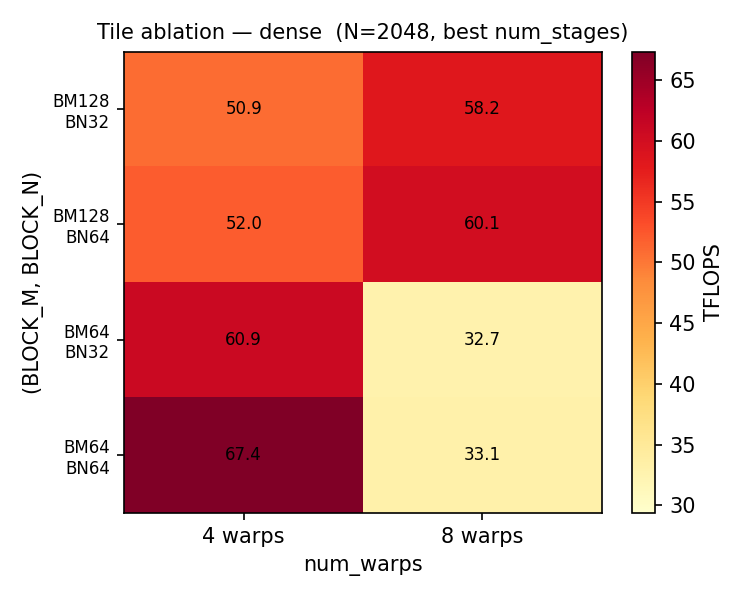
\includegraphics[width=0.45\textwidth]{../results/ablation_dense.png}
\caption{Tile ablation heatmap for dense attention at $N{=}2048$.}
\label{fig:ablation}
\end{figure}

\subsection{Roofline Analysis}

\begin{figure}[H]
\centering
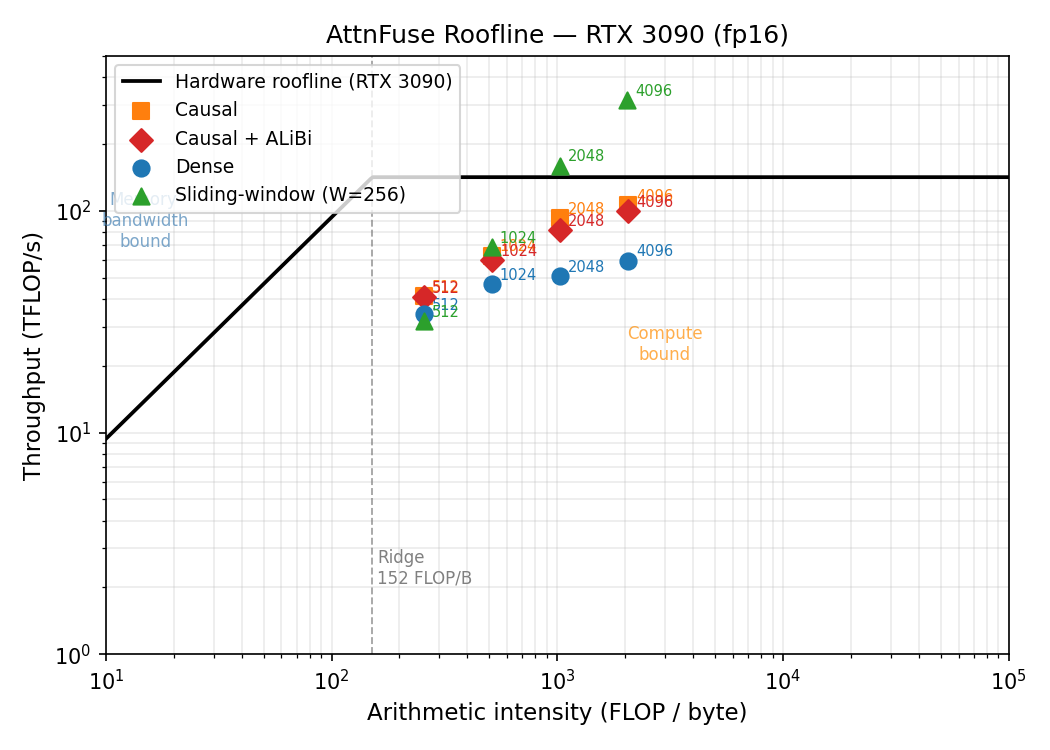
\includegraphics[width=0.45\textwidth]{../results/roofline.png}
\caption{RTX~3090 roofline: AttnFuse operating points across variants and sequence lengths.}
\label{fig:roofline}
\end{figure}

Figure~\ref{fig:roofline} places AttnFuse kernels on the hardware roofline.
Dense and causal kernels at large $N$ are compute-bound (arithmetic intensity
$>152$~FLOP/byte ridge point), explaining the plateau in throughput.
Sliding-window at small $N$ falls in the memory-bandwidth regime; as $N$
grows, the window effectively makes more of the work compute-bound and
TFLOPS rise dramatically.

\subsection{JIT Compile Time}

\begin{table}[H]
\centering
\caption{First-call JIT compile vs.\ cached dispatch latency.}
\label{tab:jit}
\small
\begin{tabular}{lrrl}
\toprule
\textbf{Variant} & \textbf{1st call (ms)} & \textbf{Cached ($\mu$s)} & \textbf{Overhead} \\
\midrule
dense         & 1812.7 & 179 & 10115$\times$ \\
causal        &  754.7 & 135 &  5605$\times$ \\
sliding\_w256 &  835.4 & 123 &  6798$\times$ \\
causal\_alibi &  823.0 & 140 &  5866$\times$ \\
causal\_rope  &   13.7 & 157 &    88$\times$ \\
\bottomrule
\end{tabular}
\end{table}

First-call cost is $\sim$0.8--1.8\,s, dominated by Triton's LLVM
compilation.  The dense variant is slower because it triggers LLVM
initialisation the first time.  \texttt{causal\_rope} is fast (13.7\,ms)
because Triton's disk cache is warm from prior runs.  After the first call,
dispatch overhead is 120--180\,$\mu$s---well below any realistic batch latency.

%% =============================================================
\section{DSL Expressibility Case Study}
%% =============================================================

To illustrate DSL productivity, we implement a \emph{relative-bias
sliding-window} variant---a mask that limits attention to a local window
combined with a learned additive bias (used in music/audio models with
local context):

\begin{lstlisting}[caption={Novel variant in 7 lines of AttnFuse DSL.}]
@af.attention
def local_biased_attn(Q, K, V):
    s = af.scaled_dot_product(Q, K)
    s = af.sliding_window(s, window_size=128)
    s = af.additive_bias(s)   # (B,H,N,N) bias
    p = af.softmax(s)
    return p @ V

# Usage: pass bias tensor at call time
out = local_biased_attn(Q, K, V, bias=rel_bias)
\end{lstlisting}

This combination---sliding-window mask + external additive bias---is not
directly available in any existing framework without a custom CUDA kernel.
AttnFuse compiles it to a single fused kernel in 0.8\,s (first call) with
no user-authored Triton code.

By contrast, the equivalent hand-written Triton kernel requires:
implementing the tiled loop structure ($\sim$80 lines), adding
sliding-window bound logic ($\sim$15 lines), adding the bias tile load
($\sim$10 lines), and tuning BLOCK\_M/BLOCK\_N manually ($\sim$half a day
on hardware).  AttnFuse reduces this to 7 user-authored lines.

%% =============================================================
\section{Related Work}
%% =============================================================

\paragraph{FlashAttention.}
Dao et al.~\cite{dao2022flashattention, dao2023flashattention2} pioneered
IO-aware tiled attention.  AttnFuse adopts the same tiled online-softmax
loop but exposes it through a composable DSL rather than a fixed kernel.

\paragraph{Triton.}
Tillet et al.~\cite{tillet2019triton} provide the JIT compilation
infrastructure we build on.  \texttt{tl.constexpr} specialisation is
central to AttnFuse's zero-overhead dispatch.

\paragraph{TVM and MLIR.}
TVM~\cite{chen2018tvm} and MLIR~\cite{lattner2021mlir} are general
tensor compiler frameworks.  They target broader hardware and operator
sets but impose significant engineering overhead; AttnFuse is intentionally
narrow (attention only) to achieve a simpler compiler with tighter
hardware-specific optimisation.

\paragraph{xFormers and Liger Kernel.}
Meta's xFormers library provides handwritten attention kernels for common
variants.  Liger Kernel provides fused Triton implementations of LLM
operators.  Neither provides a composable DSL: adding a new variant still
requires writing and tuning a new kernel.

\paragraph{ALiBi and RoPE.}
Press et al.~\cite{press2021alibi} propose ALiBi as a training-free
positional bias; Su et al.~\cite{su2021roformer} propose RoPE.
Both are first-class combinators in AttnFuse, with the fused RoPE kernel
(Section~\ref{sec:rope}) providing additional performance over the
pre-processing approach used in prior work.

%% =============================================================
\section{Limitations and Future Work}
%% =============================================================

\paragraph{Forward-only.}
AttnFuse currently compiles only the forward pass.  Backward (gradient)
computation---essential for training---would require a separate kernel
with different tile scheduling, as in FlashAttention-2's backward pass.

\paragraph{Single GPU.}
The kernel is designed for a single GPU.  Ring-attention
extensions~\cite{liu2023ring} for multi-GPU sequence parallelism would
require inter-device coordination outside the current scope.

\paragraph{Fixed head dimension.}
The \texttt{HEAD\_DIM} constexpr must be a power of two up to 256.
Variable-dimension attention (e.g., multi-query attention with grouped
key/value heads) would require a more flexible tiling strategy.

\paragraph{Triton compilation latency.}
First-call JIT cost of $\sim$1\,s is a deployment concern for latency-
sensitive serving.  Pre-compiling and caching PTX binaries to disk
(already partially done via the \texttt{\_generated/} directory) could
eliminate this in production.

%% =============================================================
\section{Conclusion}
%% =============================================================

AttnFuse demonstrates that a small, focused DSL can significantly reduce
the engineering cost of GPU attention kernel development while maintaining
near-hand-tuned performance.  With seven combinators and $\sim$1000 lines
of compiler and runtime code, it supports five production-relevant attention
variants verified by 25 correctness tests.

The key insight is that all attention variants share the same tiled
online-softmax loop structure; only the score computation, masking, bias
injection, and positional encoding differ.  By encoding these differences as
\texttt{tl.constexpr} flags, a single parameterised kernel serves all
combinations with zero runtime branching overhead.

For the two variants natively supported by PyTorch SDPA, AttnFuse achieves
79--100\% of SDPA's throughput---a modest penalty for kernel generality.
For the two variants not supported (sliding-window and causal+ALiBi),
AttnFuse provides up to $61\times$ speedup by avoiding the $\mathcal{O}(n^2)$
fallback.  The fused RoPE kernel eliminates a further 18--56\% latency
overhead relative to the pre-processing approach used in production LLMs.

%% =============================================================
\bibliographystyle{plain}
\begin{thebibliography}{99}

\bibitem{dao2022flashattention}
Tri Dao, Daniel Y. Fu, Stefano Ermon, Atri Rudra, and Christopher R\'e.
\newblock FlashAttention: Fast and memory-efficient exact attention with IO-awareness.
\newblock In \textit{NeurIPS}, 2022.

\bibitem{dao2023flashattention2}
Tri Dao.
\newblock FlashAttention-2: Faster attention with better parallelism and work partitioning.
\newblock In \textit{ICLR}, 2024.

\bibitem{tillet2019triton}
Philippe Tillet, H.~T. Kung, and David Cox.
\newblock Triton: An intermediate language and compiler for tiled neural network computations.
\newblock In \textit{MAPL at PLDI}, 2019.

\bibitem{milakov2018online}
Maxim Milakov and Natalia Gimelshein.
\newblock Online normalizer calculation for softmax.
\newblock \textit{arXiv:1805.02867}, 2018.

\bibitem{child2019generating}
Rewon Child, Scott Gray, Alec Radford, and Ilya Sutskever.
\newblock Generating long sequences with sparse transformers.
\newblock \textit{arXiv:1904.10509}, 2019.

\bibitem{press2021alibi}
Ofir Press, Noah A. Smith, and Mike Lewis.
\newblock Train short, test long: Attention with linear biases enables input length extrapolation.
\newblock In \textit{ICLR}, 2022.

\bibitem{su2021roformer}
Jianlin Su, Yu~Lu, Shengfeng Pan, Ahmed Murtadha, Bo~Wen, and Yunfeng Liu.
\newblock RoFormer: Enhanced transformer with rotary position embedding.
\newblock \textit{arXiv:2104.09864}, 2021.

\bibitem{chen2018tvm}
Tianqi Chen, Thierry Moreau, Ziheng Jiang, Lianmin Zheng, Eddie Yan, Meghan Cowan,
Haichen Shen, Leyuan Wang, Yuwei Hu, Luis Ceze, Carlos Guestrin, and Arvind Krishnamurthy.
\newblock TVM: An automated end-to-end optimizing compiler for deep learning.
\newblock In \textit{OSDI}, 2018.

\bibitem{lattner2021mlir}
Chris Lattner, Mehdi Amini, Uday Bondhugula, Albert Cohen, Andy Davis,
Jacques Pienaar, River Riddle, Tatiana Shpeisman, Nicolas Vasilache, and Oleksandr Zinenko.
\newblock MLIR: Scaling compiler infrastructure for domain specific computation.
\newblock In \textit{CGO}, 2021.

\bibitem{liu2023ring}
Hao Liu and Pieter Abbeel.
\newblock Ring attention with blockwise transformers for near-infinite context.
\newblock \textit{arXiv:2310.01889}, 2023.

\bibitem{williams2009roofline}
Samuel Williams, Andrew Waterman, and David Patterson.
\newblock Roofline: An insightful visual performance model for multicore architectures.
\newblock \textit{Communications of the ACM}, 52(4):65--76, 2009.

\end{thebibliography}

\end{document}
